\documentclass{article}
  
  % if you need to pass options to natbib, use, e.g.:
  % \PassOptionsToPackage{numbers, compress}{natbib}
  % before loading nips_2016
  %
  % to avoid loading the natbib package, add option nonatbib:
  % \usepackage[nonatbib]{nips_2016}
  
  %\usepackage{nips_2016}
  
  % to compile a camera-ready version, add the [final] option, e.g.:
  \usepackage[final]{nips_2016}
  
  \usepackage[utf8]{inputenc} % allow utf-8 input
  \usepackage[T1]{fontenc}    % use 8-bit T1 fonts
  \usepackage{hyperref}       % hyperlinks
  \usepackage{url}            % simple URL typesetting
  \usepackage{booktabs}       % professional-quality tables
  \usepackage{amsfonts}       % blackboard math symbols
  \usepackage{nicefrac}       % compact symbols for 1/2, etc.
  \usepackage{microtype}      % microtypography
  \usepackage{indentfirst}
  \usepackage{amsmath}
  \usepackage{fancyhdr}
  \usepackage{graphicx}
  \usepackage{printlen}
  
  \graphicspath{{./figures/}}
  
  \fancypagestyle{equalc}{\fancyhf{}\renewcommand{\headrulewidth}{0pt}\fancyfoot[R]{* indicates equal contribution}}
  
  \title{Faster gradient descent convergence via an adaptive learning rate schedule}
  
  % The \author macro works with any number of authors. There are two
  % commands used to separate the names and addresses of multiple
  % authors: \And and \AND.
  %
  % Using \And between authors leaves it to LaTeX to determine where to
  % break the lines. Using \AND forces a line break at that point. So,
  % if LaTeX puts 3 of 4 authors names on the first line, and the last
  % on the second line, try using \AND instead of \And before the third
  % author name.
  
  \author{
  	Satya Krishna Gorti*\\
  	University of Toronto\\
  	27 King's College Circle\\
  	Toronto, ON M5S\\
  	satyag@cs.toronto.edu
  	\And
	Mathieu Ravaut* \\ 
	University of Toronto \\
	27 King's College Circle\\
	Toronto, ON M5S\\
	mravox@cs.toronto.edu \\
}
  
  \begin{document}
  % \nipsfinalcopy is no longer used
  
  \printlength\textwidth
  
  \maketitle
  
  \begin{abstract}
    Any gradient descent requires to choose a learning rate. With deeper and deeper models, tuning that learning rate can easily become tedious and does not necesarily lead to an ideal convergence. We propose a variation of the gradient descent algorithm in the which the learning rate $\eta$ is not fixed. Instead, we learn $\eta$ itself, either by another gradient descent (first-order method), or by Newton's method (second-order). That way, gradient descent for any machine learning algorithm can be optimized. 
  \end{abstract}
  
  \thispagestyle{equalc}
  \section{Introduction}
  
  In the past decades, gradient descent has been widely adopted to optimize the loss function in machine learning algorithms \emph{ref}. Lately, the machine learning community has also used the stochastic gradient descent alternative \emph{ref}, which processes input data via batches. Gradient descent can be used in any dimension, and presents the advantage of being easy to understand and inexpensive to compute. Under certain assumptions on the loss function (such as convexity), gradient descent is guaranteed to converge to the minimum of the function. Moreover, stochastic gradient descent has proven to be very efficient even in situations where the loss functions is not convex, as is mostly the case with modern deep neural networks \emph{ref}. Other methods such as Newton's method guarantee a much faster convergence, but are typically very expensive. Newton's method for instance requires to compute the inverse of the Hessian matrix of the loss functions with regards to all parameters, which is impossible with today's hardware and today's deep networks with millions of parameters \emph{ref}. \\
  
  The quality of a gradient descent heavily depends on the choice of the learning rate $\eta$. A too high learning rate will see the loss function jumping around the direction of steepest descent, and eventually diverge. While a very low learning rate guarantees non-divergence, convergence will be very slow, and the loss function might get stuck in a local minimum. Choosing an ideal learning rate requires an intuition of the problem. Typically, researchers would start by performing a line-search over a set of different orders of magnitude of learning rates, but this is long and costly. Besides, a line-search usually assumes a fixed learning rate over time, as doing one line-search per iteration would require exponential computation cost. Usually, we see researchers setting the learning rate to an initial value then decrasing it one or a few items after training has progressed \emph{ref}.\\
  
  In this paper, we propose to automatically find the learning rate at each epoch. We still need to input an initial value, but at each iteration, our model will find a learning rate that optimizes best the loss function at this point of learning. We explore a first-order method and a second-order one to do so, with a strong emphasis on the latter. Our method could be applied to any machine learning algorithm using gradient descent. We show faster convergence on a variety of tasks and models. \\ 
  
  \section{Related work}
  
  Techniques for improving optimization of machine learning problems have a long history. The most commonly used technique is Stochastic Gradient Descent (SGD), combined with tricks like momentum \cite{polyak1964some}. While using SGD with complex neural network architectures, the non-convex nature of the problem makes it even harder to optimize. 
  
  Recently used alternatives to SGD include Contrastive Divergence \cite{hinton2006training}, Conjugate Gradients \cite{hinton2006reducing}, Stochastic Diagonal Levenberg-Marquardt \cite{lecun1998gradient}, and Hessian-free optimization \cite{martens2010deep}. All these techniques optimize the parameters of the model with the objective of minimizing a loss function. To the best of our knowledge, none of these techniques have been applied to optimize the learning rate at every iteration as we will discuss.
  
  In practice, techniques of the form $\frac{\eta}{\beta+t}$ that decay the learning rate over time are popular. The Adagrad method \cite{duchi2011adaptive} for instance divides the learning rate at each step by the norm of all previous gradients. Adadelta \cite{zeiler2012adadelta} is an extension of Adagrad that seeks to reduce its aggressive, monotonically decreasing learning rate. Adam \cite{kingma2014adam} is built on top of these methods. It stores an exponentially decaying average of past squared gradients like Adadelta, and also keeps an exponentially decaying average of past gradients, similar to momentum.
  
  LeCun et al. \cite{lecun1998gradient} mention that optimal learning rate is $\eta_{opt} = \frac{1}{\lambda_{max}}$ where $\lambda_{max}$ is the maximum eigenvalue of the Hessian matrix of the loss function with regards to all parameters. With today's neural network architectures, computing the Hessian is a computationally very expensive operation. Lecun et al. avoid computing the Hessian via approximating its eigenvalues while Martens et al. \cite{martens2010deep} estimate the Hessian via finite differences.
  
  Tom Schaul et al. \cite{schaul2013no} model the expected loss after a SGD update to deduce the best learning rate update \emph{for each dimension}. To do so, they assume a diagonal Hessian matrix. In practice, this is evidently not the case, and they rely on observed samples of the gradient to update the learning rate.
  
  Similar to Martens et al. we use finite differences to approximate first order and second order derivatives of the loss function for updating the learning rate at every iteration.
  
  
  
  \section{Adaptive learning rate}
  
  An adaptive learning gradient descent has the following schedule:\\
  \begin{align}
  w(t+1) &= w(t) -\eta(t)g(t)\\
  \eta(t+1) &= h(\eta(t))
  \end{align}
  where $g(t) = \nabla L(w(t))$, L is the loss function, w(t) represents the state of the model's weights at time t, and h is a continuous function. In the following we present several ways to update $\eta(t)$.
  
  \subsection{First-order method}
  
  The first-order method consists in doing gradient descent on the learning rate. Let's introduce a function that will be useful in the following:\\
  \begin{align}
  f : R^{n} &\rightarrow R\\
  \eta &\rightarrow L(w(t)-\eta g(t))
  \end{align}
  n corresponds to the number of learnable parameters in the model. f represents what the loss would be if we were to perform a gradient descent update with the given $\eta$.\\
  The first-order method is written:\\
  \begin{align}
  w(t+1) &= w(t) -\eta(t)g(t)\\
  \eta(t+1) &= \eta(t) - \alpha f'(\eta(t))
  \end{align} 
  This method introduces a new "meta" learning rate $\alpha$. It has the advantage of being light in cost as we only need gradients (first-order derivatives) of the loss function L. Indeed:\\
  \begin{equation}
  \forall \eta, f'(\eta) = -g(t)^{T}.\nabla L(w(t)-\eta g(t)) \text{ where . is the dot product in dimension n}
  \end{equation}
  In particular, at the value of $\eta$ used to get $w(t+1)$, we get:\\
  \begin{equation}
  f'(\eta(t)) = -g(t)^{T}.g(t+1)
  \end{equation}
  
  \subsection{Second-order method}
  
  The previous method transfers the problem of choosing an ideal learning rate for weights to choosing an ideal learning rate for the learning rate itself. To avoid that problem, the second-order method uses a Newton-Raphson algorithm:\\
  \begin{align}  
  w(t+1) &= w(t) -\eta(t)g(t)\\
  \eta(t+1) &= \eta(t) - \frac{f'(\eta(t))}{f''(\eta(t))}
  \end{align}
  Now all the learning only depends on the loss, there is no more constant value to choose. \\
  However, the second derivative of f requires building the loss Hessian matrix:\\
  \begin{equation}
  \forall \eta, f''(\eta) = g(t)^{T}.H_{L}(w(t)-\eta g(t))
  \end{equation}
  We propose to approximate this Hessian using finite differences. By using this approach on f' then f'', we get an update formula of the learning rate depending only on several values of the loss function:\\
  \begin{equation}
  f'(\eta+\epsilon) \approx \frac{f(\eta + 2\epsilon)-f(\eta)}{2\epsilon}
  \end{equation}
  \begin{equation}
  \text{and }f'(\eta-\epsilon) \approx \frac{f(\eta)-f(\eta-2\epsilon)}{2\epsilon}
  \end{equation}  
  \begin{equation}
  \text{so }f''(\eta) \approx \frac{f(\eta+2\epsilon)+f(\eta-2\epsilon)-2f(\eta)}{4 \epsilon^{2}}
  \end{equation}
  Given the finite differences on the first derivative:\\    
  \begin{equation}
  f'(\eta) \approx \frac{f(\eta+\epsilon)-f(\eta-\epsilon)}{2 \epsilon}
  \end{equation}
  We get the final simple formula for $\eta$:\\
  \begin{equation}
  \eta(t+1) = \eta(t) - 2\epsilon\frac{(f(\eta+\epsilon)-f(\eta-\epsilon))}{f(\eta+2\epsilon)+f(\eta-2\epsilon)-2f(\eta)}
  \end{equation}    
  Assuming a constant sign for the numerator, this formula means the following: when slightly increasing the learning rate corresponds to a lower loss than slightly reducing it, then the numerator is negative. In consequence, the learning rate increases, as pushing in the positive direction for the lerning rate seemed to help reducing the loss. However, reality is more complex as the sign of the denominator changes as well. 
  
  
  \subsection{BFGS}
  
  \section{Experiments}
  
  \subsection{Practical considerations}
  
  With the second-order method, the denominator in the learning rate update might underflow. To avoid such a situation, we add to the denominator a small smoothing value when it reaches zero machine, but only when it does so:\\
  \begin{align}
  \text{if } (f(\eta+2\epsilon)+f(\eta-2\epsilon)-2f(\eta)) \approx 0\\
  \text{then }\eta(t+1) = \eta(t) - 2\epsilon\frac{(f(\eta+\epsilon)-f(\eta-\epsilon))}{f(\eta+2\epsilon)+f(\eta-2\epsilon)-2f(\eta)+\delta}
  \end{align}
  A typical value of $\delta$ is $10^{-6}$. \\
  
  Besides, when updating the loss and the learning rate, one should be very careful about the order of the operations. Let's say that we just perform the \emph{k-th} iteration. We have a loss value $L^{(k)}$ and a learning rate value $\eta^{(k)}$. Then the \emph{(k+1)-th} step of our algorithm is written as follows:\\
  \begin{itemize}
  	\item Get the five loss values $f(\eta^{(k)}+\epsilon)$, $f(\eta^{(k)}-\epsilon)$, $f(\eta^{(k)}+2\epsilon)$, $f(\eta^{(k)}-2\epsilon)$ and $f(\eta^{(k)})$
  	\item $L^{(k+1)} \leftarrow f(\eta^{(k)})$
  	\item $\eta^{(k+1)} \leftarrow \eta^{(k)} -2\epsilon...$
  \end{itemize}
  
  \subsection{Results} 
  
  We compare our second-order method to a standard method, which uses a fixed learning rate schedule. In the following, this standard method will be called the \emph{basic method} That means, the basic method uses plain stochastic gradient descent as optimizer. The first order method was quite unstable. When relevant, we also include its results. We compare loss and accuracy on both training and test sets. Our goal in these experiments is not to break state of the art on the given problem, but to show an improvement in our method compared to the basic approach. 
 
  \subsubsection{Linear regression}
  
  We first tried our adaptive learning rate schedule on linear regression applied to the Boston Housing dataset \emph{ref}. This dataset of 506 points with 13 features is suitable for a simple linear regression model. 
  
  \subsubsection{Logistic regression}
  
  We also tried our method with multi-class logistic regression on the fashion MNIST dataset \emph{ref}. 
  
  \subsubsection{Image classification with neural networks}
  
  \textbf{CIFAR-10}
  
  \emph{\textbf{Second-order method}}
  
  A common benchmark in machine learning is to classify images on the CIFAR-10 dataset \emph{ref}. Deep neural networks are most suited for this task \emph{ref}. In consequence, we used a LeNet with 5 layers (2 convolutional followed by 3 fully-connected layers) and ResNet-18 \emph{ref}.
  
  We first started by optimizing the LeNet model. We trained it for different learning rate values, and 0.01 appeared to be the best choice. Thus, we compare the basic method with the second-order adaptive one starting at 0.01, using a batch-size of 32:\\
  
  \begin{figure}[!h]
  	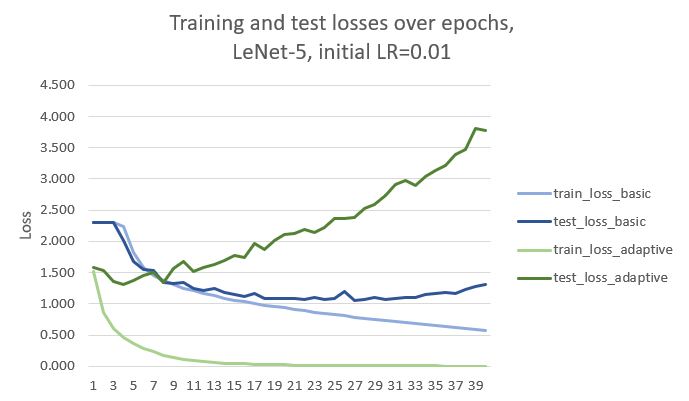
\includegraphics[width=200pt]{loss_lenet_0_01.png}
  	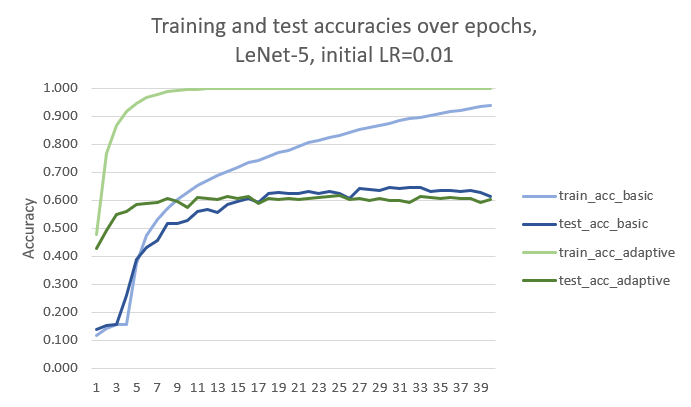
\includegraphics[width=200pt]{acc_lenet_0_01.png}
  	\caption{Second-order adaptive learning rate and basic method with LeNet, initial learning rate 0.01}
  \end{figure}

  From here we can notice three things. First, training is faster with the adaptive method. Looking at the first epochs shows that the training and test losses get optimized much quicklier than in the basic case. Then, given the values that the training loss and accuracy reach, the adaptive method is overfitting. Finally, even with this overfitting, the adaptive method plateaus around the same test accuracy than the basic method. This maximum test accuracy is reached less than 10 epochs, versus around 30 epochs for the basic method. 
  
  In the ResNet paper by \emph{ref}, ResNet is optimized via the Adam optimizer. As we are using SGD here, we added dropout (on both the basic and adaptive methods of course) at the end of the second and fourth blocks of the network to prevent overfitting. We use a batch size of 256 for training.
  
  \begin{figure}[!h]
	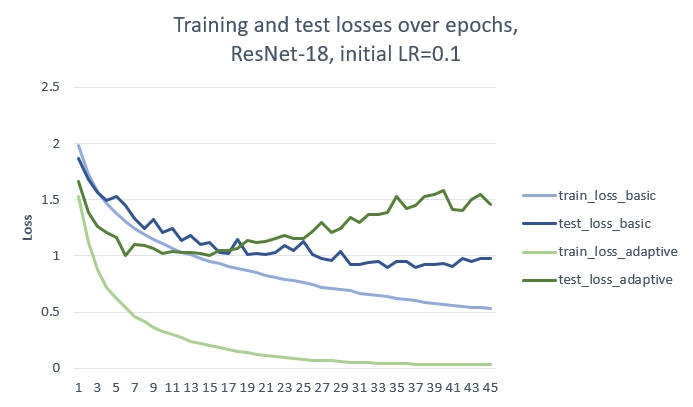
\includegraphics[width=200pt]{loss_resnet_0_1.png}
	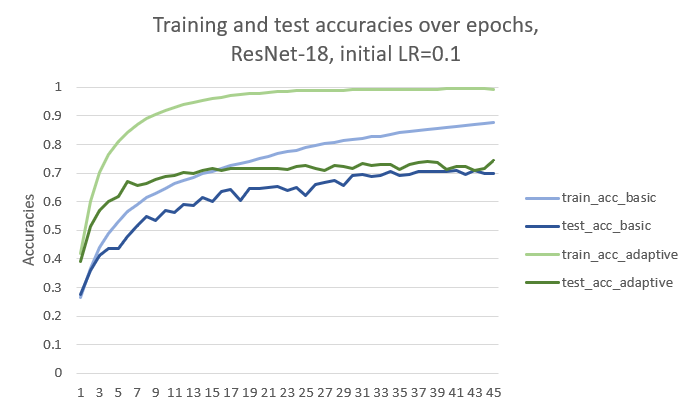
\includegraphics[width=200pt]{acc_resnet_0_1.png}
	\caption{Second-order adaptive learning rate and basic method with ResNet, initial learning rate 0.1}
\end{figure}
  
  Once again, in the adaptive schedule, all training metrics (training and test loss, training and test accuracies) are optimized faster. Typically, in the first epochs, training loss is twice lower in the adaptive version. The second-order method reaches its plateau sooner as well, after around 15 epochs versus 40 in the basic case, and then starts to overfit. Overfitting here is slightly weaker than with LeNet, probably thanks to the dropout layers. Interestingly, this time the best performance achieved by the adaptive method seems to be slightly better (74.4\%) than the best one achieved by the basic method (71\%).
  
  Let's have a look at the variations of the learning rate for both networks:
  
  \begin{figure}[!h]
	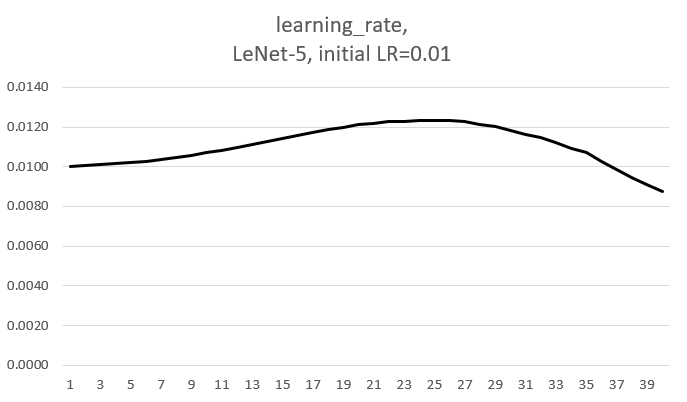
\includegraphics[width=200pt]{lr_lenet_0_01.png}
	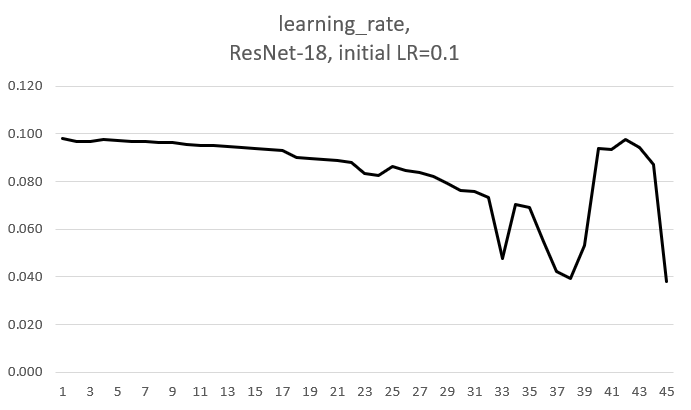
\includegraphics[width=200pt]{lr_resnet_0_1.png}
	\caption{Learning rate variations in the two previous trainings}
\end{figure}
  
  For LeNet, it seems that the initial learning rate value was a bit too low. The network increases it to boost convergence, then decreases it as training reaches its converges. With ResNet, it seems that a starting learning rate of 0.1 was a bit too high, as we see it decrease its learning rate. Something interesting starts happening here after 30 epochs, as the learning rate starts oscillating. As the loss value stops changing, it is probable that the denominator in the learning rate updates gets very small.\\
  
  Let's see what happens if we set the initial learning rate at 0.01 for the ResNet model:\\
  
  \begin{figure}[!h]
	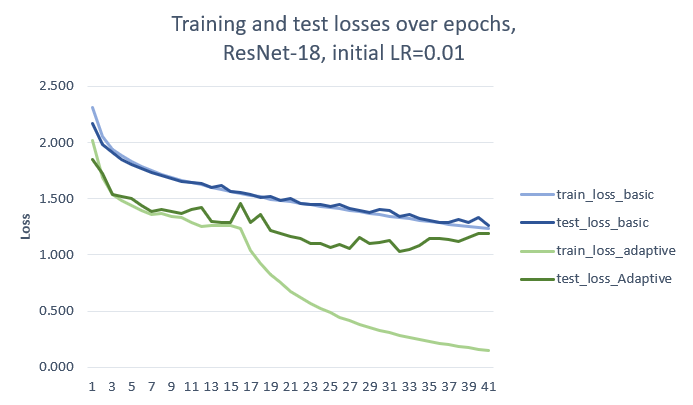
\includegraphics[width=130pt]{loss_resnet_0_01.png}
	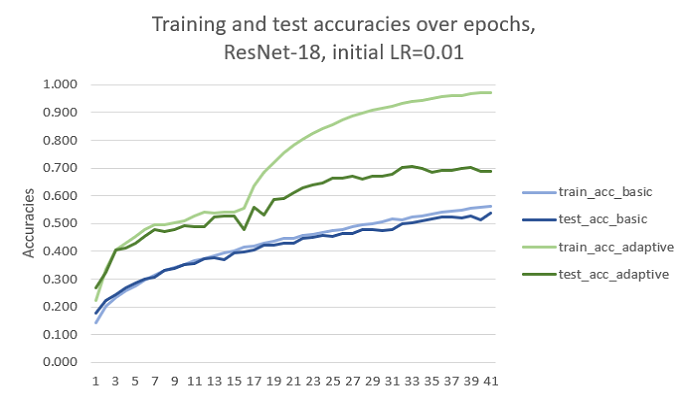
\includegraphics[width=130pt]{acc_resnet_0_01.png}
	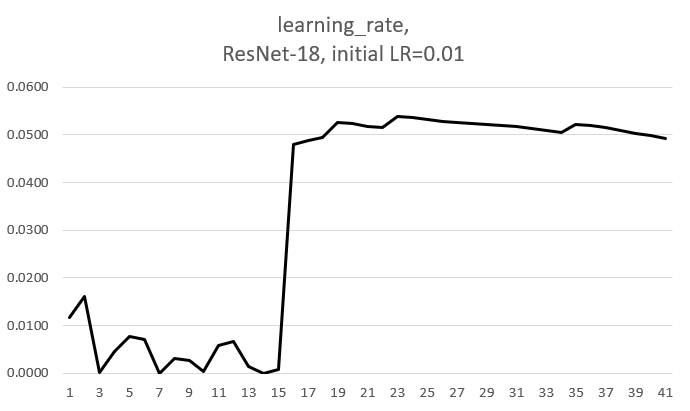
\includegraphics[width=130pt]{lr_resnet_0_01.png}
	\caption{Second-order adaptive learning rate and basic method with ResNet, initial learning rate 0.01}
\end{figure}
  
  The adaptive schedule performs consitently better than the basic one with testing accuracy being 10 to 15 points higher all the way around. This time, the initial learning rate seems to be too small, as the network increases its value until stabilizing it around 0.05, a value around the which it oscillated at the end of the previous training schedule.\\
  
  \emph{\textbf{First-order method}}
  
  Include the 3 figures of training on cifar-10 with first-order method
  
  \textbf{CIFAR-100}
  
  In this section, we increment difficulty by solving an image classification problem with 10 times more classes. After a line-search, the best learning rate to train ResNet-18 on this dataset seems to be 0.a

  figure: losses, ResNet, starting LR 0.a\\
  figure: accuracies, ResNet, starting LR 0.a\\
  figure: lr, ResNet, starting LR 0.a
  
  Once again, we see ... This time the converged value of LR is ...  
  
  \section{Further exploration}
  
  \subsection{Learning the learning rate}
  
  In the previous experiments, we have seen the learning rate converge to a given value over time. This value seems to depend on both the model and the dataset. Now a question rises: given a dataset and a model, is this value the ideal learning rate ?
  
  We started an adaptive learning rate training with the learning rate value that the ResNet model converged to in section 4.2.2 with 0.01 as a starting learning rate. 
  
  figure: losses, ResNet, starting LR 0.xx\\
  figure: accuracies, ResNet, starting LR 0.xx\\
  figure: lr, ResNet, starting LR 0.xx
  
  This time, the learning rate variations are of much weaker amplitude, as the this parameter is already in a ideal zone. 
  
  \subsection{Momentum}
  
  \subsection{Getting loss values via a validation set}
  
  \subsection{Comparison with other optimizers}
  
  In the last few years, a popular variation of gradient descent named Adam \emph{ref} has progressively gained consensus among researchers for its efficiency. Thus, we compared our method with Adam and its default learning of $10^{-3}$. 

  figure: losses, ResNet, starting LR 0.001\\
  figure: accuracies, ResNet, starting LR 0.001\\
  figure: lr, ResNet, starting LR 0.001
  
  \section{Limitations}
  
  \subsection{Choice of step $\epsilon$}
  
  In finite differences, the choice of the paramater $\epsilon$ is a main issue. Indeed, in any deep learning problem, we can expect the loss function to present noisy oscillations locally. On one hand, with a too small value of $\epsilon$, we might not capture meaningful variations of the f function. On the other hand, a too large $\epsilon$ would make the learning rate oscillate too much, reaching either too high values or even negative values. Both cases can in turn quickly make the loss function diverge. We have seen empirically that when the learning rate gets negative, training will likely not converge. All our reported experiments were done using an $\epsilon$ value of $10^{-5}$, which seemed to be a good compromise.
  
  \subsection{Choice of the initial learning rate}
  
  In our algorithm schedule, learning rate variations are automatic, but we have to choose the initial rate value. This value seems not to matter so much, as with several ranges of initial values, our algorithm still converges (to the same value).
  
  \subsection{Cost of loss computations}
  
  We have shown faster training in terms of number of epochs. However, at each iteration, we have to perform 5 back-propagations instead of one. Thus, computation time is slowed down compared to the fixed learning rate approach. \emph{show experiments results}. Assuming that the experimenter does not care about time but about finding the best loss function minimization, it is not such a big problem.
  
  \subsection{Overfitting}
  
  Our version of gradient descent reduces the training loss much faster than in the fixed learning rate approach. The training loss sometimes gets down to very surprisingly low values, while the test loss does not reduce much more than in the basic model. Thus, our model seems to be more likely to overfit. We have tried to add dropout to the ResNet model, and that proved successful. 
  
  \section{Conclusion}
  
  
  \bibliographystyle{plain}
  \bibliography{ref}
  
  
  \end{document}